\documentclass[notumble,combine]{leaflet}
\usepackage[dvipsnames,usenames]{color}
\usepackage{graphicx}
\usepackage{alltt}
\usepackage{url}
\usepackage{ascmac}
\usepackage{comment}
\usepackage{here}
\usepackage{wrapfig}

\makeatletter
% from leaflet.cls
\renewcommand\section{\@startsection{section}{1}{\z@}%
  {-3.5ex \@plus -.75ex}%
  {1ex} %{1.5ex}%
  {\normalfont\large\sectfont\color{NavyBlue}}}
\renewcommand\subsection{\@startsection{subsection}{2}{\z@}%
  {-2.5ex plus -.5ex}%
  {1\p@} %{1ex}%
  {\normalfont\normalsize\sectfont\color{BrickRed}}}
\makeatother

\graphicspath{{figures/}} 

\title{
	\vfill
	\includegraphics[width=\textwidth]{kbug-logo}
	\vfill
	\resizebox{\linewidth}{!}{\bf 関西*BSDユーザ会}%
	\\[\baselineskip]
        \resizebox{\linewidth}{!}{{\bf \url{http://www.kbug.gr.jp/}}}
	\vfill
        \resizebox{2cm}{!}{\textcolor{red}{\bf{@}}}
	\vfill
	\includegraphics[width=\textwidth]{banner2008}
        \resizebox{\linewidth}{!}{{\bf \url{http://k-of.jp/2008/}}}\\
        \resizebox{\linewidth}{!}{2008年11月7日(金),8日(土)}
}

\date{}

\begin{document}
\maketitle
\thispagestyle{empty}
\pagebreak{}
\section{関西*BSDユーザ会ってなに?}
関西 *BSD ユーザ会 (Kansai *BSD Users Group; K*BUG)とは、
BSD系OSのユーザ同士の情報交換のための{\em 場}で、1999年に作
成されました。

年に数度(大体2ヶ月に1度程度)の勉強会や宴会を行っています。

\subsection{K*BSDの基本理念}
K*BUGの基本理念は以下のようになっています
(\url{http://www.kbug.gr.jp/charter.html}より)。

\fbox{\begin{minipage}{\textwidth}
\begin{itemize}
\item 場の提供を目的とする
\item 人のケツは叩くが足は引っ張らない
\item 来るものは拒まず、猿ものは追わず
\item だれでも役員になれる。誰でも役員は止められる
\end{itemize}
\end{minipage}}
\begin{wrapfigure}[8]{r}{3cm}
\begin{center}
 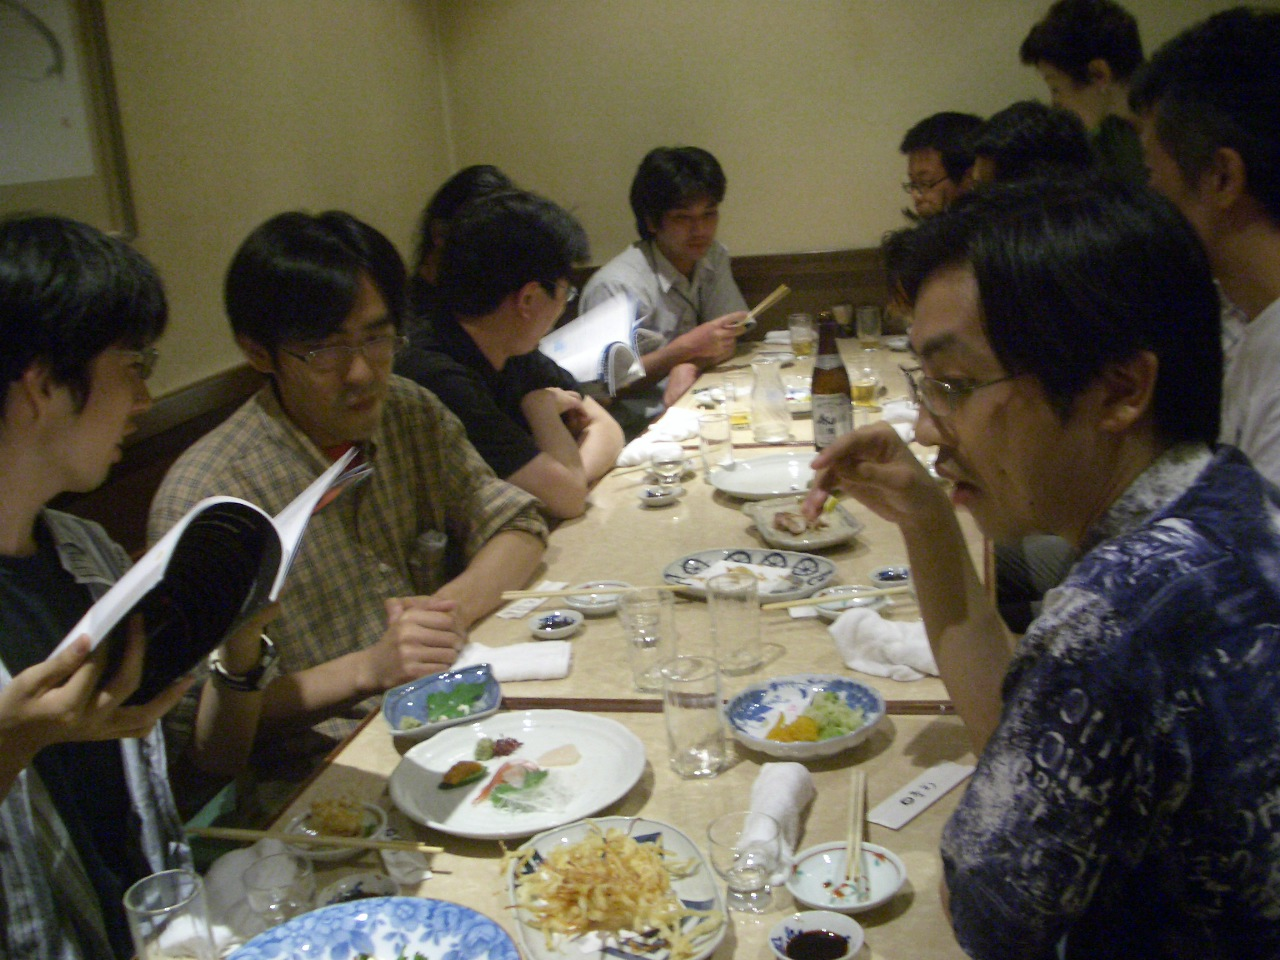
\includegraphics[width=3cm]{CIMG2521}\\
 飲み会は大切
\end{center}
\end{wrapfigure}

少し難しく感じるかもしれないですが、\textcolor{red}{BSDへの愛と情熱}があれば、
あなたが\textcolor{blue}{やりたいと思うことができる場}がK*BUGなのです。

また、メンバーは色々な技術に詳しいですし、技術に関する話も大好きなので、
あなたの疑問などもぶつけてみてください。

\section{最近の活動}
KOF2007からの最近の活動とその内容は以下のとおりです。

もし、興味のあるテーマがあるようでしたら、是非一度遊びにきてください。

\subsection{2008年9月6日(土)@大阪}
\begin{itemize}
\item iPod touchを使った何か
\item はじめようNetwork Audio
\item perlでログインプロキシ
\item Typolight WebCMSの概要
\item ぼくのなつやすみ2008(未完)
\item 懇親会: 四季彩
\end{itemize}
\subsection{2008年8月13日(土) OSC2008 Kansai@京都}
\begin{wrapfigure}{r}{3cm}
\begin{center}
 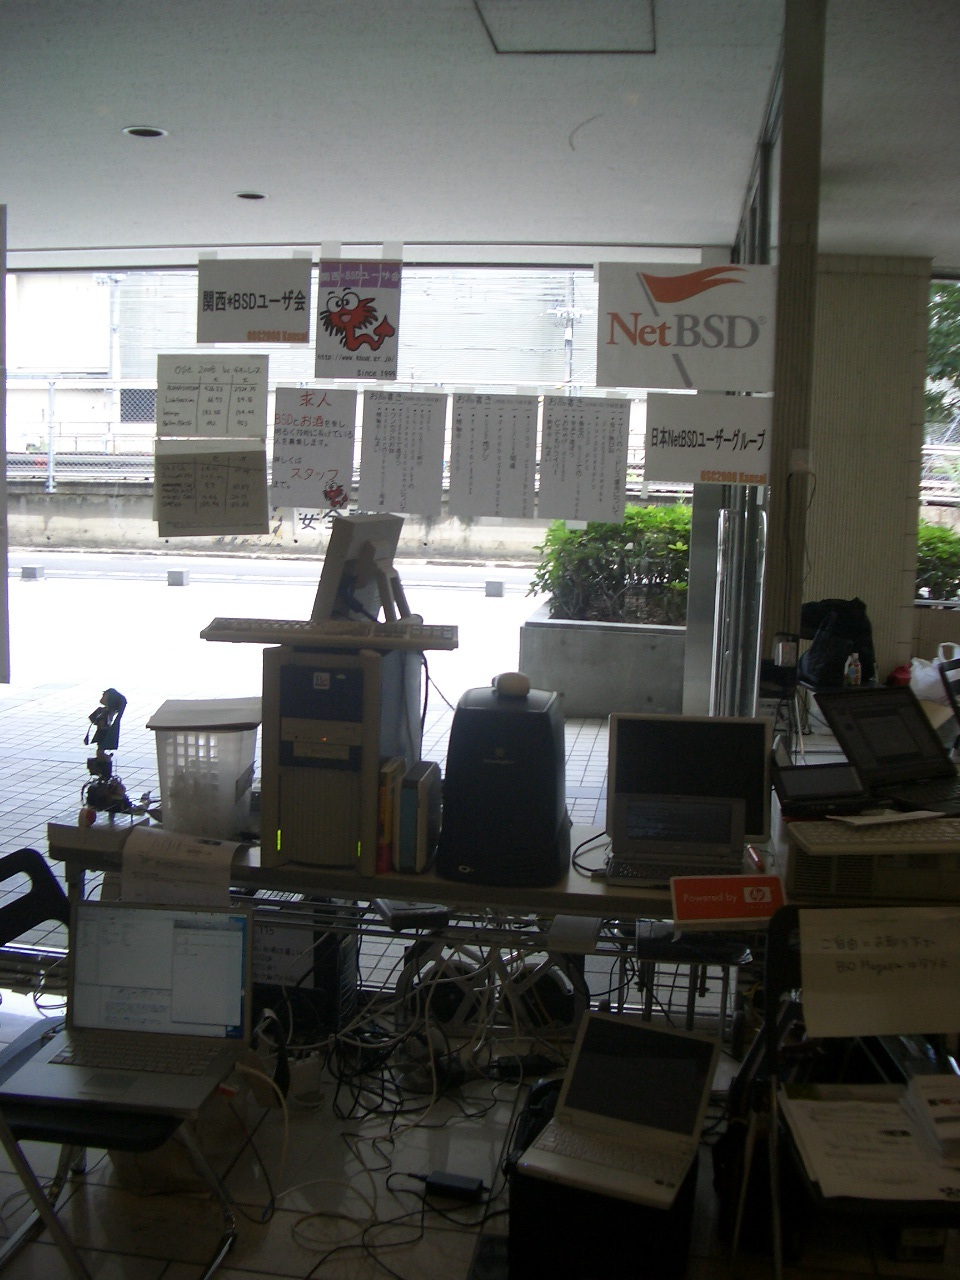
\includegraphics[width=3cm]{CIMG2018}%\\
 %OSC2008 Kansaiブースの様子
\end{center}
\end{wrapfigure}

OSC2008 Kansai\footnote{\url{http://www.ospn.jp/osc2008-kansai/}}で、JNUGさんと共同ブースを設置しました。

\begin{itemize}
\item NetBSDなひととき
\item 展示
\begin{itemize}
\item BeBox (NetBSD化失敗)
\item NetBSD/O2
\item ネギ降りサーボ + FT232を使ったLCDパネル
\item 魅惑のえびじゅんコレクション
\item Squeak/MGL2@NetBSD/hpcmips
\end{itemize}
\item ブース企画
\begin{itemize}
\item bcbench \footnote{\url{http://www.yagoto-urayama.jp/~oshimaya/nbug/etc/bench/bcbench.html}}チキンレース
\item 夏の京都恒例:電力測定
\end{itemize}
\end{itemize}
\subsection{2008年7月13日(土)@京都}
\subsection{2008年5月17日(土)@京都}
\begin{itemize}
\item ZFS
\item NanoBSD紹介
\item ThinkPad X61のSuspend/Resumeについて
\item FT245で遊ぼう
\item ワンセグのお話
\item DebianのOpenSSL関連
\item 懇親会:んまい
\end{itemize}
\subsection{2008年3月15日(土)@大阪}
\begin{itemize}
\item iPod jailbreak
\item iSCSI関連
\item freebsd-update
\item USB地デジ
\item twitter-API
\item 懇親会 %:????
\end{itemize}

\subsection{2008年2月9日(土)@京都}
\begin{itemize}
\item Life with dtrace
\item サーバのヘッドレス運用について
\item 負け組日記 FreeBSD/amd64
\item kurobox-pro + LCD pro
\item 最近の(BSDでの)Squeak
\item 音声で遊ぼう
\item おみやげ: HD-30 どこでもドライバー
\item 新年会:んまい
\end{itemize}

\begin{center}
 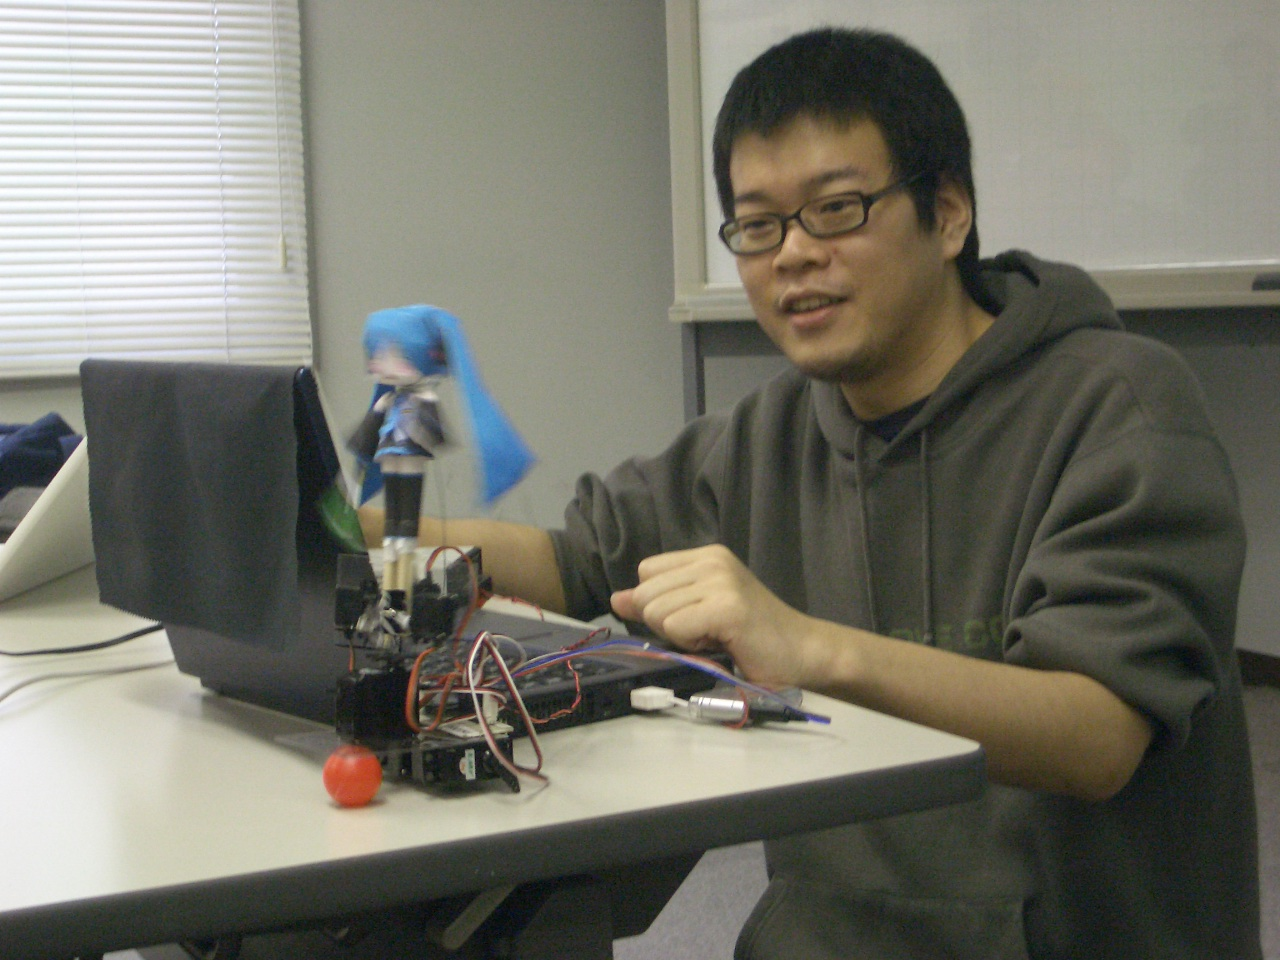
\includegraphics[width=4cm]{CIMG0535}\\
 勉強会での発表: ネギ振りサーボ
\end{center}

\subsection{2007年12月8日(土)@大阪}
\begin{itemize}
\item 総会
\item 忘年会 %:???
\end{itemize}
\subsection{2007年11月10日(土)@KOF2007に合流}
\begin{itemize}
\item JNUGブースに合流%???
\item 懇親会%:???
\end{itemize}
\subsection{その他}
以下のようなURLで、メンバーの発表が紹介されていますので、活動内容を知るために参考にしてください。
\begin{itemize}
 \item \url{http://hp.vector.co.jp/authors/VA012337/misc/presentation.html}
 \item \url{http://qml.610t.org/FreeBSD/BUG.html}
\end{itemize}

\section{K*BUG@KOF2008}
\subsection{展示}
\begin{itemize}
 \item 魅惑のえびじゅんコレクション
 \item ○○セグ @ \{Net,Free\}BSD
 \item \{Net,Open\}BSD/sparc
 \item 固 (Hardware?)
 \begin{itemize}
  \item Gainer\footnote{\url{http://gainer.cc/}}, Arduino\footnote{\url{http://arduino.cc/}}, DWM 2008/05基板 @ FreeBSD
  \item 参考出品: AVR\footnote{\url{http://sacraya.610t.org/Press/No9/avr/}}, MAX232
 \end{itemize}
 \item 響 (sound?)
 \begin{itemize}
  \item ネコミミサーボシステム\footnote{\url{http://www.rogiken.org/daemon/works.html}}
  \item 世界聴診器\footnote{\url{http://swikis.ddo.jp/WorldSthethoscope/2}}
  \item audioオシロスコープ\footnote{\url{http://xoscope.sourceforge.net/}}
 \end{itemize}
 \item BSD Magazine(not ASCII)\footnote{\url{http://www.bsdmag.org/}}展示
 \item \textcolor{red}{\Large 他にもたくさんの○○BSDが…}
\end{itemize}

\section{BSDに関する情報}
\subsection{リンク集}
\begin{itemize}
\item JNUG(Japan NetBSD Users Group)\\
  今回ご一緒にブースを出させていただきました(\_o\_)\\
  \url{http://www.jp.netbsd.org/}
\item FreeBSD友の会  \url{http://www.jp.freebsd.org/}
\item OpenBSD本家  \url{http://www.openbsd.org/ja/}
\end{itemize}

\pagebreak{}
\section{これからの関連イベント(予定)}
詳細は、Webページをご確認ください。

\begin{itemize}
\item 2008年12月 6日(土) 	定期総会+第7回研究会+忘年会@大阪
\item 2009年 3月12日(木)-15(日) AsiaBSDCon 2009 \footnote{\url{http://2009.asiabsdcon.org/}}
\end{itemize}

\section{BSDなひととき}
以下のようにBSDなひとときをおこないますので、ご参加ください。

\begin{itemize}
\item 日時: 2008/11/07 17:00-17:50
\item 会場: 9F-セミナールーム1
\item 講師: 蛯原 純 (株式会社創夢/The NetBSD Project)
\item 主催:日本NetBSDユーザーグループ
\item \url{http://k-of.jp/2008/list_seminar.html#23}
\end{itemize}

\begin{comment}
BSD系UNIXを取り巻く環境と、将来の展望について議論し、 BSDコミュニティ間の情報交換を行なうBOFセッションです。
4.4BSDの流れをくむFreeBSD/NetBSD/OpenBSDなど、 BSD系UNIXのユーザグループ合同で、BSD系UNIX全般を対象とした幅広いテーマで議論します。
\end{comment}

\vfill

\begin{minipage}{\textwidth}
\begin{boxnote}

\section{kbug-usersメーリングリスト}
K*BUGでは、K*BUGメンバーの情報交換や、イベントなどの情報伝達用に
kbug-usersメーリングリストを用意しています。

K*BUGメンバーは、基本的にはこのメーリングリストを読んでいることが期待
されます。

購読は以下のURLをご参照ください。
\begin{itemize}
 \item \url{http://www.kbug.gr.jp/maillist.html}
\end{itemize}
\end{boxnote}
\end{minipage}

\end{document}  
